% Last update/Última versão: 11/Sep/2016
%%%%%%%%%%%%%%%%%%%%%%%%%%%%%%%%%%%%%%%%%%%%%%%%%%%%%%%%%%%%%%%%%%%%%%
%=====================================================================
% 							Pacotes Fundamentais
%=====================================================================
\documentclass[
% -- op\c{c}\~{o}es da classe memoir --
12pt,				% tamanho da fonte
openright,			% cap\'{\i}tulos come\c{c}am em p\'{a}g \'{\i}mpar (insere p\'{a}gina vazia caso preciso)
oneside,			% para impress\~{a}o em verso e anverso. Oposto a oneside
a4paper,		% tamanho do papel.
% -- op\c{c}\~{o}es da classe abntex2 --
%chapter=TITLE,		% t\'{\i}tulos de cap\'{\i}tulos convertidos em letras mai\'{u}sculas
%section=TITLE,		% t\'{\i}tulos de se\c{c}\~{o}es convertidos em letras mai\'{u}sculas
%subsection=TITLE,	% t\'{\i}tulos de subse\c{c}\~{o}es convertidos em letras mai\'{u}sculas
%subsubsection=TITLE,% t\'{\i}tulos de subsubse\c{c}\~{o}es convertidos em letras mai\'{u}sculas
% -- op\c{c}\~{o}es do pacote babel --
english,			% idioma adicional para hifeniza\c{c}\~{a}o
%french,			% idioma adicional para hifeniza\c{c}\~{a}o
%spanish,			% idioma adicional para hifeniza\c{c}\~{a}o
brazil,				% o \'{u}ltimo idioma \'{e} o principal do documento
%sumario=tradicional,
]{article}
\usepackage[a4paper, 
right = 1.5cm, left = 3.5cm, top = 3cm, bottom = 2cm]{geometry}
\usepackage[utf8]{inputenc}
\usepackage[english,portuguese]{babel}
%\usepackage[myheadings]{fullpage}
\usepackage[T1]{fontenc}
\usepackage{graphicx, setspace}
\usepackage{booktabs}
\usepackage{sectsty}
\usepackage{url}
\usepackage{mathptmx}
\usepackage{comment}
\usepackage{multirow}
\usepackage{graphicx}
\usepackage[table,xcdraw]{xcolor}
\usepackage{enumitem}
\usepackage{blindtext}
\usepackage{float}
\usepackage{tikz}
\usetikzlibrary{calc,trees,positioning,arrows,chains,shapes.geometric,%
	decorations.pathreplacing,decorations.pathmorphing,shapes,%
	matrix,shapes.symbols,through}
\usepackage[bottom]{footmisc}
\usepackage{pdfpages}
\usepackage{caption} % \caption*
\usepackage{csquotes}
\usepackage{footnote} % Permite footnote em tabelas


%=====================================================================
% 							Pacotes Bibliográficos
%=====================================================================

\usepackage[backend=biber,
	style = abnt,%
	noslsn, %
	extrayear, %
	uniquename=init,% 
	giveninits, %
	justify, %
	sccite,% 
	scbib, %
	repeattitles, %
	doi=false,isbn=false,url=false, 
	maxcitenames=3]{biblatex}
\addbibresource{./refs.bib}

\renewenvironment{quote}
{\small\list{}{\fontsize{10pt}{12pt}\singlespacing\rightmargin=0cm \leftmargin=4cm}%
	\item\relax}
{\endlist}

%=====================================================================
% 							Comandos específicos da FAPESP
%=====================================================================
%=========================================================================
 %                             Novos Comandos
 %=========================================================================
\newcommand{\HRule}[1]{\rule{\linewidth}{#1}}
\onehalfspacing
\setcounter{tocdepth}{3}
\setcounter{secnumdepth}{3}

\newcommand{\titulo}[1]{\def\meuTitulo{#1}}
\newcommand{\tituloIngles}[1]{\def\meuTituloIngles{#1}}
\newcommand{\numFAPESP}[1]{\def\numFAP{#1}}
\newcommand{\tipoRelatorio}[1]{\def\tipoRelat{#1 }} %o espaço depois do #1 é importante
\newcommand{\autor}[1]{\def\nomeAutor{#1}}
\newcommand{\cidade}[1]{\def\nomeCidade{#1}}
\newcommand{\universidade}[1]{\def\nomeUniversidade{#1}}
\newcommand{\faculdade}[1]{\def\nomeFaculdade{#1}}
\newcommand{\periodoVigencia}[1]{\def\periodVig{#1}}
\newcommand{\periodoRelatorio}[1]{\def\periodRelat{#1}}
\author{Gabriel Petrini da Silveira}
\date{Julho de 2018}

\newcommand{\Figure}[1]{Figura~\ref{fig:#1}}
\newcommand{\Table}[1] {Tabela~\ref{#1}}
\newcommand{\Equation}[1] {Equa\c{c}\~ao~\ref{#1}}
\newcommand{\addFigure}[3] { %Parametros scale, fig_name, caption 
    \begin{figure}[!hbt]
      \centering
      \includegraphics[scale=#1]{figures/#2}
      \caption{#3}\label{fig:#2}
    \end{figure}
}

%=========================================================================
 %                             Capa-Título
 %=========================================================================

\newcommand{\geraTitulo}{
\clearpage
\begin{titlepage}
  \begin{center}
      \vspace*{-3cm}
      { \setstretch{.5} 
        \textsc{\nomeUniversidade} \\
        \HRule{.2pt}\\
        \textsc{\nomeFaculdade}
      }

      \vspace{5.5cm}

      \Large \textbf{\textsc{\meuTitulo}}
	  \HRule{1.5pt} \\ [0.5cm]
      \linespread{1}
      \large Projeto de Pesquisa para Solicitação  de Auxílio à Pesquisa Regular na modalidade Mestrado, fomentado pela Fundação de Amparo à Pesquisa do Estado de São Paulo. \\ 
  	   \HRule{1.5pt} \\ [0.5cm]
%       Projeto FAPESP \texttt{\#\numFAP}
       
       Candidato: \nomeAutor
         \\ [0.1cm]
       Orientador: Lucas Azeredo da Silva Teixeira
       \\ [0.1cm]
       %Co-orientador: Franklin Leon Perez Serrano
       \vfill
       {\normalsize  \nomeCidade, Julho de 2018}
\end{center}
\end{titlepage}
}
%=========================================================================
 %                             Fonte-Headings
 %=========================================================================
\usepackage{titlesec}
\titleformat{\chapter}{\normalfont\LARGE\bfseries}{\thechapter}{1em}{}
\titlespacing*{\chapter}{0pt}{3.5ex plus 1ex minus .2ex}{2.3ex plus .2ex}
\newcommand{\chapterbreak}{\let\clearpage\relax}

\addto\captionsportuguese{\renewcommand{\contentsname}{Sumário}}
\addto\captionsportuguese{\renewcommand{\bibname}{Referências bibliográficas}}

%=========================================================================
 %                             Resumo e Abstract
 %=========================================================================
\newcommand{\Resumo}[1]{
   \begin{otherlanguage}{portuguese}
       \begin{abstract} \thispagestyle{plain} \setcounter{page}{2}
          #1
        \end{abstract}
   \end{otherlanguage} 
} %end \Resumo


\newcommand{\Abstract}[1]{
   \begin{otherlanguage}{english}
      \begin{abstract} \thispagestyle{plain} \setcounter{page}{3}
       #1
      \end{abstract}    
    \end{otherlanguage} 
} %end \abstract

%=========================================================================
 %                             Folha de rosto
 %=========================================================================

%=========================================================================
 %                             Informações gerais do projeto
 %=========================================================================
%INFORMAÇÕES GERAIS DO PROJETO. Não é necessário para uma proposta de projeto

\newcommand{\folhaDeRosto}{
   \section*{Informações Gerais do Projeto}
   \begin{itemize}
      \item Título do projeto: 
            \begin{itemize}\item[] \textbf{\meuTitulo} \end{itemize}
      \item Nome do candidato: 
            \begin{itemize}\item[]\textbf{\nomeAutor}\end{itemize}
      \item Nome do orientador:
                  \begin{itemize}\item[]\textbf{Lucas Azeredo da Silva Teixeira}\end{itemize}
      \item Instituição sede do projeto: 
            \begin{itemize}
               \item[]\textbf{\nomeFaculdade \ da \nomeUniversidade} 
            \end{itemize}
   \end{itemize}
}

\newcommand{\folhaDeRostoEN}{
	\clearpage
	\section*{General project information}
	\begin{itemize}
		\item Project title: 
		\begin{itemize}\item[] \textbf{\meuTitulo} \end{itemize}
		\item Applicant's Name: 
		\begin{itemize}\item[]\textbf{\nomeAutor}\end{itemize}
		\item Supervisor's Name:
		\begin{itemize}\item[]\textbf{Lucas Azeredo da Silva Teixeira}\end{itemize}
		\item Project Institution: 
		\begin{itemize}
			\item[]\textbf{\nomeFaculdade \ da \nomeUniversidade} 
		\end{itemize}
	\end{itemize}
}
%=====================================================================
% 							Outros Pacotes
%=====================================================================
\usepackage[colorinlistoftodos]{todonotes}
\usepackage{subfigure}
\usepackage{setspace}
\usepackage{lipsum}  
\usepackage{amsmath} % Para cases
\usepackage[cm]{fullpage}

%=====================================================================
% 							Página de título e folha de rosto
%=====================================================================
%-----
% Página de título
% Observação: As definições que aparecem a seguir comporão a
%             página de título e a folha de rosto.
%-----
%% Define o nome da universidade onde o projeto foi desenvolvido.
\universidade{Universidade Estadual de Campinas}
%
%% Define o nome da faculdade onde o projeto foi desenvolvido.
\faculdade{Instituto de Economia}
%
%% Define o título do projeto.
\titulo{Título}
%
%
%% Define o autor do relatório.
\autor{}
\cidade{Campinas}


\begin{document}
%=====================================================================
% 							Numeração pré-textual
%=====================================================================
\pagenumbering{roman}
%=====================================================================
% 							Folha de título
%=====================================================================
%\geraTitulo
%=====================================================================
% 							Folha de rosto
%=====================================================================
% Gera a folha de rosto.
%\folhaDeRosto
%=====================================================================
% 							Título
%=====================================================================
\begin{center}
\rule{\textwidth}{1.2pt}
	Projeto de Tese para Doutorado em Ciência Econômica\\
	%\textbf{Investimento residencial, instituições e crescimento: Uma análise comparativa a partir de um modelo supermultiplicador sraffiano com consistência entre fluxos e estoques}
	\textbf{\Large{Macroeconomia imobiliária: \\\large{uma análise comparada}}}\\
	\textbf{Gabriel Petrini da Silveira}
\rule{\textwidth}{1.2pt}
\end{center}
%=====================================================================
% 							Resumo
%=====================================================================
\Resumo{
	A crise imobiliária de 2007 --- que se tornou uma crise financeira global --- demarcou mudanças importantes na teoria econômica. Dentre elas, destaca-se a guinada de parte da literatura para a compreensão das implicações macroeconômicas do investimento residencial. 
	Apesar destes esforços recentes, muitas questões estão em aberto. 
	Da revisão de literatura, verifica-se a necessidade de se investigar as relações entre mercado imobiliário e de bolha de ativos.
	Adicionalmente, a literatura que conecta investimento residencial com as teorias de crescimento lideradas pela demanda é escassa e precisa ser mais explorada.
	Partindo de 17 países da OCDE e de forma a suprir estas lacunas, a presente pesquisa irá:
		(i) investigar quais os condicionantes institucionais que permitem uma maior participação das hipotecas no balanço patrimonial dos bancos (``hipotecarização'') por meio de uma análise qualitativa comparativa com lógica \textit{fuzzy} (fsQCA);
		(ii) avaliar os determinantes macroeconômicos do investimento residencial no pós-década de 70 através de um modelo de dados em painel dinâmico e; 
		(iii) desenvolver um modelo supermultiplicador sraffiano com consistência entre fluxos e estoques para integrar os condicionantes e determinantes do investimento residencial e avaliar suas implicações para a dinâmica. 
		Ao considerar elementos qualitativos e quantitativos de forma comparada, o estudo visa
		evidenciar mecanismos que conectam bolha de ativos e dinâmica macroeconômica e seus efeitos sobre a composição patrimonial dos diferentes setores institucionais.
		O entendimento dos condicionantes, determinantes e implicações da hipotecarização pode auxiliar políticas econômicas mais eficazes em conciliar
		crescimento econômico, estabilidade e regulação financeira. 
		\\\\
\noindent\textbf{Palavras-chave:} Investimento residencial; Supermultiplicador sraffiano; metodologia de consistência entre fluxos e estoques; Análise Qualitativa Comparativa; Lógica \textit{fuzzy}.
}
%=====================================================================
% 							Abstract
%=====================================================================
\begin{comment}
Habilitar caso seja necessário um abstract em outra página

\Abstract{
teste in english
}
\end{comment}
%=====================================================================
% 							Numeração textual
%=====================================================================
\pagenumbering{arabic}

%=====================================================================
% 							Formatação título seção
%=====================================================================
\sectionfont{\scshape}

%=====================================================================
% 							Corpo de texto
%=====================================================================
\linespread{1.5}
\doublespacing
% Controle do espaçamento entre um parágrafo e outro:
\setlength{\parskip}{0.2cm}  % tente também \onelineskip
\begingroup
\let\clearpage\relax
\section{Introdução e Justificativas}\label{Intro}


%=============================================================================
% 							INTRODUÇÃO
%=============================================================================

%GFC E QUESTIONAMENTO DO INVESTIMENTO COMO CAUSA CAUSANS

%INTRODUÇÃO MAIS LONGA: EUA E CRISE

A crise \textit{subprime} de 2008, antes uma crise focalizada no mercado imobiliário americano, ampliou-se em uma crise financeira que tomou dimensões globais. Além das mudanças sócio-econômicas, a crise teve implicações para a teoria econômica. Se, por um lado, abalou a macroeconomia ortodoxa ao ponto da política fiscal estar sendo repensada \cite{blanchard_rethinking_2017}, por outro, redirecionou algumas pautas na heterodoxia. Distribuição e desigualdade, temas tão caros a esta última tradição, ganharam novo fôlego\footnote{Cabe pontuar que até o \textit{mainstream} passou a se dedicar ao assunto com destaque ao trabalho de \textcite{piketty_o_2014}.} \cites{carvalho_personal_2016}{ederer_will_2019} enquanto parte da literatura passou a destacar o consumo como um dos possíveis motores de crescimento\footnote{Para uma resenha da literatura recente sobre o consumo, ver \textcite{brochier_macroeconomics_2017}}. Paralelamente, verificou-se um crescente interesse nas implicações macroeconômicas do investimento residencial \cites{teixeira_crescimento_2015}{fiebiger_semi-autonomous_2018} e é justamente nesta agenda de pesquisa que essa investigação se insere. 

Apesar da relevância do investimento residencial para a dinâmica macroeconômica não se restringir aos EUA, parte expressiva desta literatura tem centrado esforços neste caso em específico. A razão disso é que os imóveis são  uma das formas de riqueza mais comuns entre as famílias norte-americanas e serviam --- principalmente nos anos 2000 --- de colateral para tomada de crédito \cite{teixeira_uma_2011} MAIS REFERÊNCIAS. A forma de ``realizar'' o ganho de capital com a bolha imobiliária que ocorreu no período, sem precisar liquidá-los, era justamente ampliando o endividamento à medida que este colateral aumentava de valor \cite{teixeira_crescimento_2015}. 
%Nesses termos, evidencia-se os impactos da inflação de imóveis sobre a demanda agregada. 

Da revisão de literatura, verificou-se que a fronteira tem avançado em três frentes. Uma delas diz respeito a importância das instituições para a compreensão dos impactos deste gasto para a dinâmica macroeconômica enfatizando as relações entre mercado imobiliário, de crédito e endividamento das famílias.
Outra frente trata da importância do investimento residencial para a dinâmica macroeconômica por meio de modelos econométricos.  
Por fim, uma parcela menor direciona esforços para conectar o investimento das famílias nas teorias de crescimento. Esta pesquisa irá avançar nestas direções e suprir algumas das lacunas que serão destacadas adiante.


Compreendido este panorama, a presente investigação tem como objetivo estudar o papel macroeconômico dos imóveis.
Em particular, pretende-se analisar as relações entre mercado imobiliário e de crédito tendo em vista elementos teóricos, empíricos e institucionais. 
A justificativa desta investigação se deve a uma regularidade do capitalismo contemporâneo pouco estudada: aumento repentino da hipotecas no balanço patrimonial dos bancos (hipotecarização).
Dito isso, esta pesquisa busca responder a seguinte pergunta: quais os condicionantes, determinantes e implicações da hipotecarização sobre a dinâmica macroeconômica?
Para tanto, parte-se de uma abordagem comparativa multidimensional: (i) qualitativa; (ii) quantitativa e; (iii) integrada.
Cada uma destas frentes será discutida a seguir.



\subsection{Qualitativa: Especificidades institucionais da macroeconomia imobiliária}


DEFINIÇÃO DE INSTITUIÇÃO

APRESENTAR HIPOTECARIZAÇÃO

Uma análise que complementa os efeitos do investimento residencial sobre a dinâmica financeira é a da aqui denominada de ``hipotecarização''. 
Desenvolvida por \textcite{jorda_great_2014}, esta hipótese destaca a crescente participação das hipotecas nos balanços patrimoniais dos bancos de ao menos 17 países da OCDE\footnote{\textcite{jorda_great_2014} também destacam que o crédito hipotecário era concedido fora do sistema bancário até os 1900 e isso dificulta a estimação dos dados.}\footnote{Paralelamente, os autores pontuam que os empréstimos às famílias têm aumentado a uma velocidade superior ao valor de seus ativos e, portanto, verifica-se uma maior alavancagem --- logo, maior fragilidade financeira das famílias --- apesar do aumento do preço dos imóveis.} (ver figura \ref{GraficoJorda}).
Apesar de esclarecer as relações entre investimento residencial (lado real) e balanço patrimonial dos bancos (lado financeiro), tal contribuição não tem sido investigada sob um ponto de vista pós-keynesiano em que as relações financeiras entre os diferentes agentes institucionais desempenham um papel central. Para ilustrar a compatibilidade desta hipótese a esta tradição, tal contribuição permite destacar os efeitos do investimento residencial sobre a dinâmica financeira: 

\begin{quote}
	\textit{To a large extent the core business model of banks in advanced economies today resembles that of real estate funds: banks are borrowing (short) from the public and capital markets to invest (long) into assets linked to real estate.} [...] \textit{looking more deeply at the composition of bank credit, it becomes clear that the rapid growth of \textbf{mortgage lending} to households has been the \textbf{driving force} behind this remarkable change in the composition of banks’ balance sheets} \cite[p.~2, grifos adicionados]{jorda_great_2014}
\end{quote}
Além disso, a partir da base de dados desenvolvida --- e em constante atualização --- pela equipe de Jordà, uma investigação mais aprofundada desta hipótese abre uma agenda de pesquisa sobre a importância do investimento residencial para a dinâmica macroeconômica que vai além dos EUA e se estende para alguns países da OCDE. Nesses termos, a presente pesquisa se justifica pela necessidade de uma maior compreensão 
%do papel das hipotecas no sistema bancário bem como 
da relação entre investimento residencial e dinâmica macroeconômica dados os impactos reais e financeiros que este componente da demanda agregada tem sobre o ciclo econômico. 

\begin{figure}[H]
	\centering
	\caption{Participação do empréstimo imobiliário no total do balanço patrimonial dos bancos (1870-2016)}
	\label{GraficoJorda}
	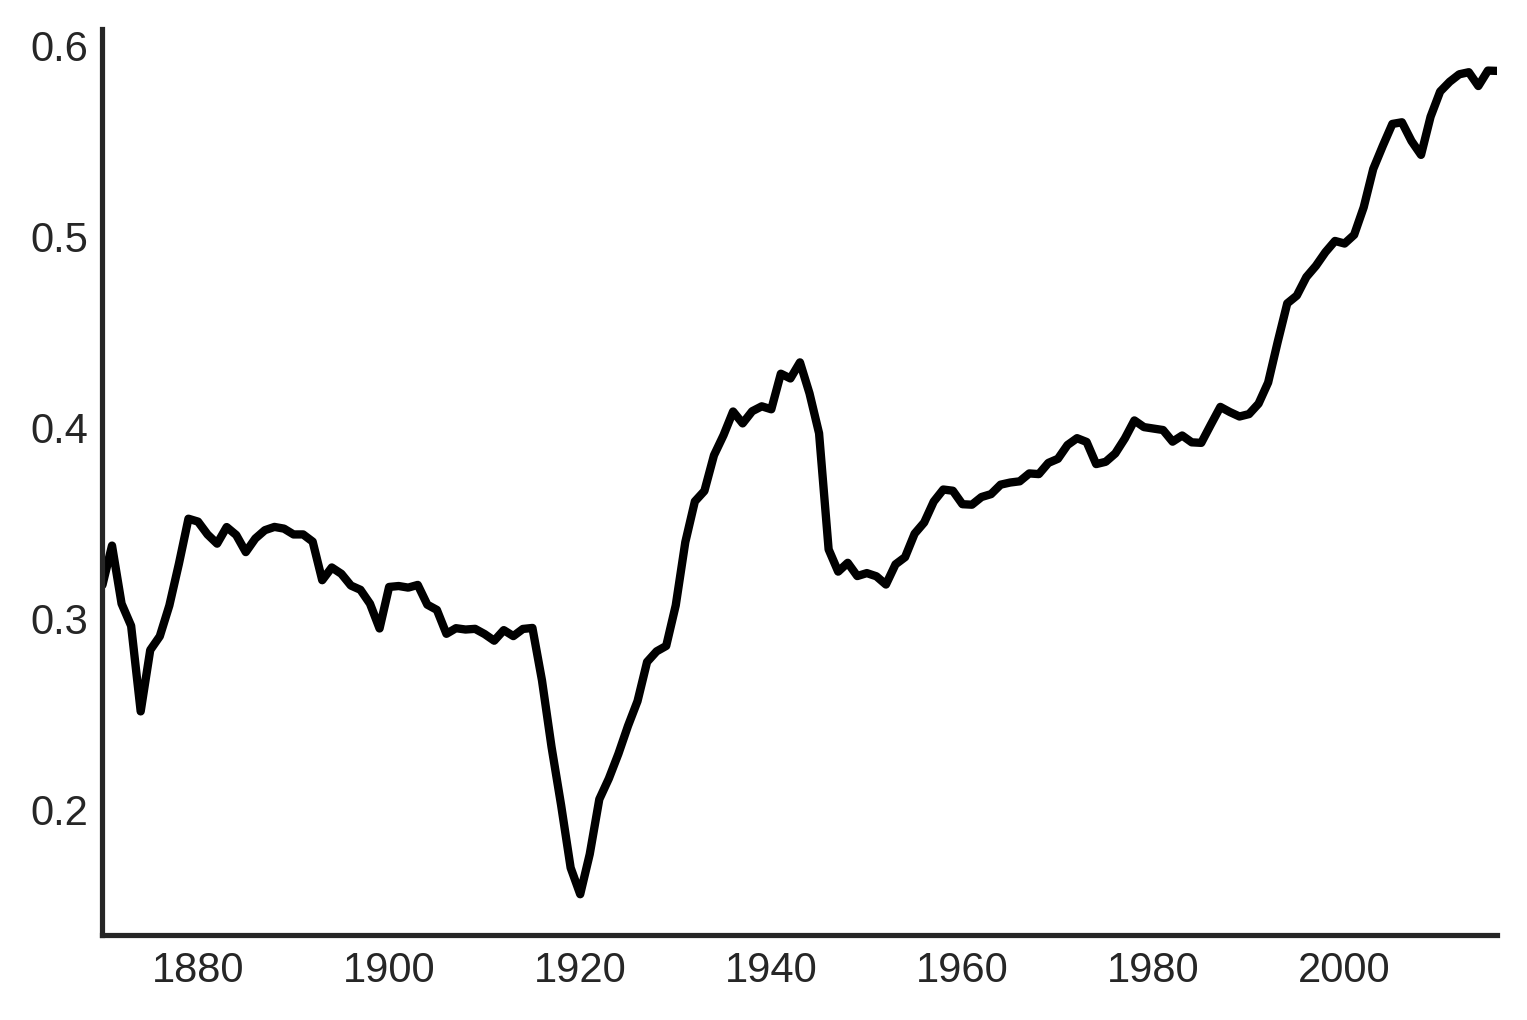
\includegraphics[width=.65\textwidth]{Jorda_Mean.png}
	\caption*{\textbf{Fonte:} \textcite[p.~10]{jorda_great_2014}}
\end{figure}





ELEMENTOS INSTITUCIONAIS



A título de exemplo, \textcite{wijburg_alternative_2017} destacam que a especificidade institucional do mercado imobiliário alemão\footnote{Os autores também apontam que os preços dos imóveis na Alemanha estagnaram enquanto o resto do mundo presenciou um aumento. No entanto, observa-se um movimento recente de aumento nos preços no país, indicando uma maior relevância do tema em um futuro próximo.} o configura como um contra ponto ao norte-americano:

\begin{quote}
	\textit{On the one hand, the German housing
		market was one of the few markets in Western Europe that was not severely affected by the
		global housing boom of the early 2000s. On the other hand, recent developments suggest
		that the role of finance in the German housing system is \textbf{changing}, but not in the same way as
		in other countries}. \cite[p.~969, grifos adicionados]{wijburg_alternative_2017}
\end{quote}
Também seguindo uma análise das instituições, \textcite{van_gunten_varieties_2018} argumentam que as mudanças institucionais ocorridas desde a década de 90 foram responsáveis pela maior intensificação financeira das famílias\footnote{Isto é, maior endividamento das famílias e não um aumento no número de famílias endividadas.} em Portugal e Espanha se comparado com França e Alemanha. Sendo assim, para uma melhor compreensão das inter-relações entre o mercado imobiliário e o de crédito, se faz necessário destacar a importância das instituições\footnote{
	Ao longo desta pesquisa, adota-se a definição de instituições como em 	DEFINIÇÃO DE INSTITUIÇÕES}.  


%INSTITUIÇÕES

A pluralidade de resultados reportada acima sugere que a especificidade institucional de cada país desempenha um papel central nas implicações macroeconômicas do investimento residencial e, portanto, carece de uma investigação mais detalhada.





: (i) possibilidade de transferência de riscos (\textit{e.g.} securitização\footnote{Para uma descrição do aumento da securitização nos Estados Unidos, ver \textcite{green_american_2005} e \textcite{cagnin_o_2009}. Destaca-se também o aumento desta prática entre os países europeus \cite{european_central_bank_housing_2010}.}); (ii) disponibilidade de crédito de longo-prazo para as famílias \cite{schwartz_politics_2009}; (iii) duração das hipotecas e existência de um mercado secundário \cite{green_american_2005}; (iv) determinação  e tipo da taxa de juros das hipotecas (fixa ou flexível); (v) arranjo regulatório sobre reembolso antecipado (contrato ou legislação) e formas de refinanciamento e; (vi) permissividade da retirada do capital próprio (\textit{equity withdrawal contracts})\footnote{Dentre os itens elencados anteriormente, destaca-se o acesso a linhas de crédito através das hipotecas cuja relevância é maior para o caso norte-americano --- pelos efeitos significativos já mencionados sobre o ciclo econômico --- e por serem mais incomuns nos países europeus \cite[p.~95]{van_gunten_varieties_2018}}.

\begin{table}[htb]
	\centering
	\caption{Características institucionais de alguns países europeus da OCDE}
	\label{Institucional}
		\resizebox{.7\textwidth}{!}{%
			\begin{tabular}{c|c|c|c|c|c|c}
				\hline\hline \\
				\multirow{2}{*}{\textbf{Países}} & \multicolumn{6}{c}{\textbf{Características institucionais}} \\\cline{2-7}
				&
				\textbf{\begin{tabular}[c]{@{}c@{}}Maturidade\\ Hipotecária\\(meses)\end{tabular}} &
				\textbf{\begin{tabular}[c]{@{}c@{}}Taxa de juros\\ Hipotecária\end{tabular}} &
				\textbf{\begin{tabular}[c]{@{}c@{}}Reembolso antecipado:\\ Contratado (C)/\\ Legislado (L)\end{tabular}} &
				\textbf{\begin{tabular}[c]{@{}c@{}}Possibilidade de segunda\\hipoteca a partir\\da valorização do imóvel\end{tabular}} &
				\textbf{\begin{tabular}[c]{@{}c@{}}Financiamento pelo\\ Mercado de capitais (\%)\end{tabular}} &
				\textbf{\begin{tabular}[c]{@{}c@{}}Execução\\ Hipotecária\\(meses)\end{tabular}} \\\hline
				\textbf{Alemanha}                & 30   & Fixa       & C/L   & Não permitido    & 14   & 9    \\\hline
				\textbf{Espanha}                 & 30   & Variável   & C/L   & Limitado         & 45   & 8    \\\hline
				\textbf{França}                  & 19   & Fixa       & C/L   & Não permitido    & 12   & 20   \\\hline
				\textbf{Holanda}                 & 30   & Fixa       & C     & Permitido        & 25   & 5    \\\hline
				\textbf{Itália}                  & 22   & Variável   & L     & Não permitido    & 20   & 56   \\\hline
				\textbf{Portugal}                & 40   & Variável   & L     & Sem informação   & 27   & 24  \\\hline
				\hline
				
			\end{tabular}%
		}
	\caption*{\textbf{Fonte:}  \textcite[p.~94, adaptado e traduzido]{van_gunten_varieties_2018}}
\end{table}



\subsection{Quantitativa: Implicações dinâmicas do investimento residencial}

LER ARTIGO DO BUNDESBANK


No que diz respeito ao ciclo econômico, parte da literatura econométrica também tem lançado luz sobre a importância do investimento residencial e tal relevância não se restringe à crise \textit{subprime} nem aos EUA. \textcite{alvarez_does_2010}, por exemplo, concluem que tal tipo de investimento antecede o ciclo econômico para o caso espanhol e resultados semelhantes podem ser encontrados para França, Espanha  e Itália enquanto o caso alemão apresenta uma dinâmica distinta \cites{ferrara_cyclical_2010}{ferrara_common_2010}. 
Outros estudos empíricos, por sua vez, têm enfatizado o efeito riqueza --- via valorização dos imóveis --- sobre o consumo e indicam tais canais de transmissão são mais incidentes, em ordem, sobre Estados Unidos e Grã Bretanha e mais brandos no caso francês e alemão \cites{sastre_assessment_2010}{chauvin_wealth_2010}{bassanetti_effects_2010}{arrondel_housing_2010}.

ALÉM DO CICLO

\subsection{Integrada: Dimensão real e financeira do mercado imobiliário}

Uma vez que a dívida hipotecária é o principal componente do endividamento das famílias \cite{van_gunten_varieties_2018}, se faz necessária uma melhor compreensão da conexão entre o investimento residencial com as formas de financiamento e estoques financeiros de forma integrada.
Nesses termos, a abordagem SFC se mostra a mais adequada para o tipo de análise pretendido. Portanto, fica evidenciada a lacuna que esta pesquisa procurará preencher.
Sendo assim, um modelo de crescimento do tipo SSM com a metologia SFC (adiante, SSM-SFC) se mostra como uma alternativa para tratar do investimento residencial em que são mapeadas as relações financeiras entre os diferentes agentes institucionais.



Pontuada a importância do investimento residencial e a relevância das instituições para compreendê-lo, cabe inspecionar a forma com que a heterodoxia tratou do tema. Parte significativa desta literatura  --- emergente no pós-crise imobiliária --- centra esforços na conexão deste tipo de gasto com processos mais gerais como a financeirização \cites{aalbers_financialization_2008}{bibow_financialization_2010}
enquanto uma fração minoritária o relaciona com as variabilidades
de capitalismo com o \textit{welfare state} \cite{schwartz_politics_2009}. No
entanto, a partir da revisão bibliográfica, verificou-se que uma fração pequena da literatura heterodoxa aborda as relações entre crescimento e investimento residencial.
Um  exemplo é o trabalho de \textcite{zezza_u.s._2008} em que são investigados os efeitos da diminuição --- apesar da distribuição da renda a favor dos lucros --- da propensão média a poupar da economia norte-americana por meio da introdução do mercado imobiliário na metodologia SFC\footnote{
	Tal resultado, argumenta, decorre dos ganhos de capital nos mercados imobiliário e acionário entre o topo da distribuição, contribuindo para a diminuição da taxa de poupança.
}. 
Por mais que este trabalho seja uma via para a inclusão do investimento residencial nos modelos macroeconômicos, tal gasto não é o principal determinante da dinâmica  uma vez que parte de uma especificação kaleckiana do investimento das firmas.
Sendo assim, a influência do investimento das famílias para a dinâmica é bastante limitada.

Alguns trabalhos seguiram a contribuição de \textcite{zezza_u.s._2008}.
Um deles é o de \textcite{nikolaidi_securitisation_2015} com dois tipos de agentes demandando imóveis: parcela dos trabalhadores e investidores institucionais.
Para os primeiros, a demanda por casas é determinada positivamente pela poupança deste setor acrescido de empréstimos hipotecários e negativamente pelo preço dos imóveis de modo que não pode ser considerado estritamente autônomo.
Já os demais agentes, demandam imóveis tal como outros ativos financeiros, ou seja, depende positivamente de sua taxa de retorno.
Em conjunto, tais equações comportamentais determinam que a taxa de crescimento do investimento residencial depende tanto da razão entre a demanda por imóveis em relação ao total quanto de sua inflação que, por sua vez, é determinada pelo estoque de imóveis não vendidos.
Sendo assim, o investimento residencial no trabalho de \textcite{nikolaidi_securitisation_2015} possui tanto uma parcela autônoma em relação à renda quanto outra induzida pela renda disponível das famílias.
No entanto, ao partir do procedimento de \textcite{godley_money_1999} para determinação do portfólio de ativos dos agentes, trata os imóveis como um ativo financeiro qualquer sem considerar suas particularidade, qual seja, durabilidade e baixo risco. %TODO: Rever particularidade dos imóveis.

Outra vertente heterodoxa tem lançado mão de modelos baseados em agentes (ABM) para avaliar as relações entre instabilidade financeira, endividamento das famílias e distribuição de renda.
Em linha com \textcite{cynamon_inequality_2013} e \textcite{erlingsson_integrating_2013}, \textcite{cardaci_inequality_2018} parte da hipótese de consumo cascata de \textcite{veblen_theory_1899} e \textcite{duesenberry_income_1949} --- retomada por \textcite{frank_expenditure_2014} --- para conectar a concentração da renda ao aumento do preço dos imóveis.
%\footnote{Dentre as contribuições, vale pontuar a endogeinização de um mercado (e rede) de crédito com consumo financiado por empréstimos colateralizados por hipotecas --- como em \textcite{mian_house_2011} --- como uma fonte alternativa de financiamento que compensa a estagnação salarial.}.
Apesar de relevante, tal contribuição não avança em direção a uma especificação dos determinantes da taxa de crescimento do investimento residencial e, portanto, deve-se prosseguir na busca de alternativas na heterodoxia.

A partir desta revisão da literatura de crescimento que inclui investimento residencial, 
conclui-se que estes modelos estão mais centrados nas consequências e menos nos determinantes do investimento residencial de modo que pouco avançaram em seu tratamento teórico.
Uma forma de incluir esse gasto nos modelos de crescimento heterodoxos é a de \textcite{teixeira_crescimento_2015} --- retomada em \textcite{da_silveira_investimento_2019} --- em que é utilizado um modelo supermultiplicador sraffiano (SSM em inglês) por estabelecer um padrão de crescimento liderado pela demanda em que os gastos autônomos não criadores de capacidade produtiva (ditos improdutivos) determinam a taxa de crescimento de longo prazo. 

Uma forma de conectar o investimento residencial com o modelo do supermultiplicador sraffiano é por meio da taxa de juros real dos imóveis desenvolvida por \textcite{teixeira_crescimento_2015} definida como taxa de juros hipotecária deflacionada pela inflação de imóveis. 
Nesta formulação, a taxa de juros das hipotecas capta o serviço da dívida para os ``investidores'' (neste caso, famílias) enquanto a variação do preço dos imóveis permite incorporar mudança no patrimonio líquido\footnote{Em linhas gerais, esta taxa real de juros aufere de modo satisfatório o custo real em imóveis de se comprar imóveis \cite[p.~53]{teixeira_crescimento_2015}. Tal proposta, portanto, lança luz sobre a influência da inflação imobiliária na construção de novos imóveis e, de acordo com o SSM, na determinação do nível e da taxa de crescimento do produto.}. 
A partir deste tipo específico de taxa de juros real, portanto, é possível introduzir inflação de ativos nos modelos do tipo SSM. No entanto, a referida taxa foi desenvolvida para examinar a bolha de ativos ocorrida nos EUA e, portanto, não foi feita uma investigação a despeito da aplicabilidade para outros países e este é um dos objetivos desta pesquisa.


Outro modelo que une o SSM a metodologia SFC é o de \textcite{da_silveira_investimento_2019}. Tal contribuição, apesar de analisar a dinâmica de dois tipos distintos de estoques de capital (das firmas e das famílias), carece de uma relação entre o mercado imobiliário e de crédito, bem como composição patrimonial dos bancos.


Como será discutido adiante, a abordagem SFC é compatível inúmeras teorias e propostas apesar do arcabouço contábil rígido\footnote{Apenas para ilustrar a pluralidade de temas que tal metodologia já abordou, temos --- mesmo que em sua forma mais originária encontrada em \textcite{godley_macroeconomics_1983} --- as formas de financiamento das firmas \cites{asimakopulos_kalecki_1983}{skott_finance_1988}{messori_financing_1991}; endogeneidade da moeda e importância do sistema bancário \cites{messori_financing_1991}{dow_horizontalism:_1996}{arestis_theoretical_1996}{godley_money_1999}; endividamento, distribuição de renda e, apenas para restringir os temas, financeirização \cites{palley_inside_1996}{wolfson_irving_1996}{palley_money_1997}{palley_financial_2002}{dos_santos_revisiting_2009}{palley_inside_2010}{hein_finance-dominated_2012}.}. 
A mesma variabilidade de temas possíveis de serem abordados pela metodologia SFC se estende para a pluralidade dos ativos passíveis de serem incorporados e ao grau de complexidade financeira de cada modelo. Uma forma de visualizar tal flexibilidade é por meio da figura \ref{Heatmap} em que são mapeados os ativos mais frequentes. No entanto, esta figura também revela que a literatura não dá a devida atenção aos imóveis\footnote{Deve ser pontuada a notória exceção de \textcite{zezza_u.s._2008} em que é apresentado um modelo com imóveis em um aparato kaleckiano enfatizando as implicações distributivas mas não trata de questões envolvendo ganhos de capital ou dos determinantes do investimento residencial.}, sendo o ativo menos estudado. 



\begin{figure}[htb]
	\centering
	\caption{Mapa de calor dos ativos modelados com SFC}
	\label{Heatmap}
	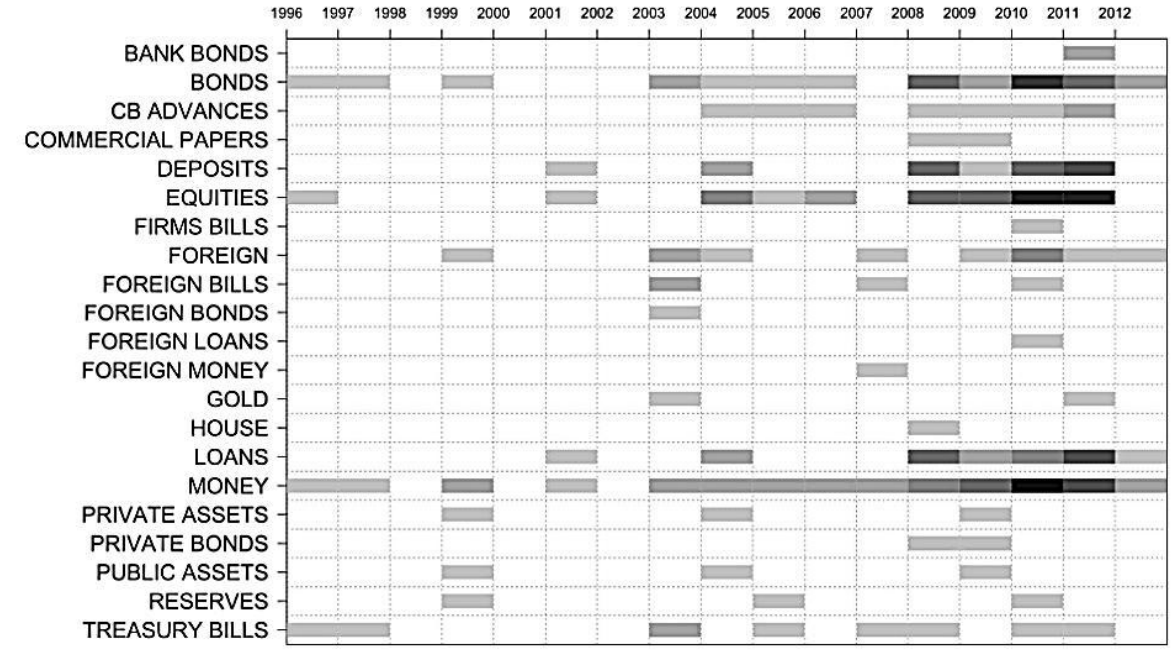
\includegraphics[width = 0.9\textwidth]{/dados/Dissertacao/Escrita_Dissertacao/Da_Silveira_Dissertacao_Atual/Modelo/Caverzassi_Heatmap.png}
	\caption*{\textbf{Fonte:} \textcite[p.~4]{caverzasi_stock-flow_2013}}
\end{figure}



Compreendidas tais relações, será desenvolvido um modelo SSM-SFC para dar conta das relações entre lado real e financeiro da economia.
Portanto, esta pesquisa segue o caminho aberto por \textcite{brochier_supermultiplier_2018} ao adicionar um tratamento adequado das relações financeiras no SSM por meio da metodologia SFC estentendo as contribuições de: 
(i) \textcite{jorda_great_2014} ao investigar o processo de ``hipotecarização'' sob um prisma pós-keynesiano a partir de uma análise qualitativa comparativa (QCA); 
%(ii) \textcite{serrano_sraffian_1995} ao incluir o investimento residencial na agenda de pesquisa do supermultiplicador sraffiano; 
(ii) \textcite{teixeira_crescimento_2015} ao avaliar a aplicabilidade da taxa própria de juros dos imóveis para além dos Estados Unidos e;
(iii) \textcite{da_silveira_investimento_2019} ao conectar as relações entre o mercado imobiliário e de crédito diante das especificidades institucionais destacas anteriormente por meio de um modelo SFC de simulação. 


\begin{comment}
Nos Estados Unidos (EUA), o início dos anos 2000 é marcado por momentos bastante distintos. Logo em 2001, a economia é atingida pela crise das bolhas-ponto-com com a possibilidade de uma recessão. No entanto, a recuperação foi rápida e seguida de um ciclo de crescimento que se estendeu de 2002 a 2007 \cite{cagnin_o_2007}.  Por mais que a economia americana seguiu crescendo até 2007, o investimento residencial iniciou a reversão já em 2005. Ao longo deste período, os demais componentes da demanda agregada contribuíram para o adiamento da crise, mas não foram suficientes para impedir o colapso do investimento residencial ocorrido em 2008. 
Apesar desta dinâmica sugerir uma atipicidade, segue um padrão bem definido para o caso norte-americano, qual seja, o ciclo econômico é liderado pelo investimento residencial \cites{green_follow_1997}{leamer_housing_2007}{fiebiger_trend_2017}\footnote{
Ao avaliar o caso norte-americano, \textcite{green_follow_1997} conclui que o investimento residencial antecipa o ciclo econômico, mas que isso não implica no estabelecimento de uma relação causal. 
}.

Neste ponto, cabe mencionar o ineditismo de \textcite{green_follow_1997} e \textcite{leamer_housing_2007} --- revisitado em \textcite{leamer_housing_2015} e por \textcite{fiebiger_semi-autonomous_2018} --- ao lançar luz sobre a importância do investimento residencial na determinação dos ciclos econômicos nos EUA em todo o pós-guerra.
Antes mesmo da crise no mercado imobiliário,
\textcite{leamer_housing_2007} destaca a capacidade preditiva e relação causal  do investimento residencial com o PIB. Sucintamente, afirma que a construção de novos imóveis permite, via aumento das linhas de crédito, um maior consumo de bens duráveis e, portanto, o ciclo econômico americano pode ser configurado como um \textit{consumer cycle} e não como um \textit{business cycle}.




Vale ressaltar que a partir do estabelecimento do SSM, algumas questões são colocadas: quais são esses gastos autônomos e quais seus determinantes? Qual o padrão de financiamento e suas consequências? \textcite{pariboni_household_2016} e \textcite{fagundes_dinamica_2017}, por exemplo, avançaram em detalhar o consumo financiado por crédito.  \textcite{brochier_supermultiplier_2018}, por sua vez, incorporam o SSM em uma estrutura contábil mais completa, o arcabouço de consistência entre fluxos e estoques (SFC, na sigla em inglês), para compreender a dinâmica do consumo a partir da riqueza. 

Nesta família de modelos: 
(i) o grau de utilização converge ao grau normal (planejado pelas firmas) no longo prazo; 
(ii) a distribuição renda não influencia o crescimento de longo prazo; 
(iii) o investimento das \textbf{firmas} segue o princípio de ajuste do estoque de capital e;
(iv) o ajuste do estoque de capital é feito de forma tênue e gradual. 


\end{comment}
\section{Objetivos}\label{OBJ}

O \textbf{objetivo geral} da tese é investigar as implicações macroeconômicas do mercado imobiliário e suas relações com as instituições, inflação de ativos e instabilidade financeira. 
% tendo em vista sua relevância macroeconômica. 
Parte-se de uma abordagem multidimensional para contemplar seus principais elementos teóricos e empíricos, visando integrar o lado real ao financeiro dando a devida atenção às instituições. %, são eles: (i) institucionais; (ii) dinâmicos e; (iii) integração do lado real e financeiro.
Cada objetivo específico é o desdobramento de uma dessas dimensões da assim chamada macroeconomia imobiliária cujas metodologias e procedimentos são detalhados na seção seguinte. 

O \textbf{primeiro} objetivo específico consiste em examinar as configurações institucionais que determinam o grau de hipotecarização do sistema bancário de um país a partir de uma análise qualitativa comparada (do inglês, QCA). A partir deste modelo, é possível encontrar as condições necessárias e suficientes para explicar o porquê de alguns sistemas bancários possuírem uma maior participação relativa das hipotecas nos balanços das instituições financeiras.
%A importância desta contribuição também se dá pela possibilidade de extrapolar o potencial explicativo de tais configurações institucionais para além dos países presentes na base de dados de \textcite{jorda_rate_2019} e inferir os respectivos graus de hipotecarização.

O \textbf{segundo} objetivo específico é explorar alguns fatos estilizados da macroeconomia imobiliária e, em particular,  estimar os determinantes do investimento residencial tendo em vista sua relevância para a dinâmica macroeconômica. 
A importância deste modelo é uma melhor compreensão da relação entre investimento residencial, concessão de crédito e bolha de ativos. %a possibilidade de se investigar as implicações do investimento residencial para o endividamento das famílias; preço dos imóveis; crescimento econômico e estabilidade financeira.
Para tanto, desenvolve-se um modelo de séries temporais em painel para os países presentes na base de dados de \textcite{jorda_rate_2019}. 

Por fim, o \textbf{terceiro} objetivo específico é avaliar as implicações macroeconômicas de um sistema bancário ativo com racionamento de crédito por meio de um modelo AB-SFC de simulação com famílias heterogêneas e investimento residencial explicitamente modelado. 
Desse modo, ao integrar o lado real e financeiro da macroeconomia imobiliária é possível desenvolver um modelo teórico no qual o financiamento dos imóveis desempenha um papel central.
Este modelo permitirá análises mais elaboradas dos efeitos das bolhas de ativos na demanda agregada; taxa de crescimento econômico; endividamento das famílias (heterogêneas); composição patrimonial dos bancos e; estabilidade financeira.
%Além disso,  uma melhor compreensão da heterogeneidade das famílias para a dinâmica dos fluxos e dos estoques permite investigar a ``Nova Narrativa''. 


\begin{comment}
\begin{description}
	\item[Objetivo geral] Investigar as implicações macroeconômicas dos imóveis.
	\item[Objetivos específicos] {\color{white}Teste}
	\begin{itemize}
		\item Examinar as configurações institucionais da ``hipotecarização'';
		\item Estimar os principais determinantes macroeconômicos do investimento residencial;
		\item Avaliar as implicações de um sistema bancário ativo e de bolha de ativos com ciclo de crédito endógeno por meio de um modelo AB-SFC com famílias heterogêneas e investimento residencial autônomo.
	\end{itemize}
\end{description}
\end{comment}

\section{Metodologia}\label{passos}


Para atender os objetivos, a pesquisa será dividida em três capítulos independentes.
O primeiro deles trata das relações entre o mercado imobiliário e de crédito a luz das especificidades institucionais por meio de uma análise qualitativa comparativa.
No capítulo seguinte, será estimado um painel macrodinâmico para analisar os determinantes do investimento residencial.
Em seguida, CAPÍTULO SFC
 
 
A hipótese de trabalho do primeiro capítulo é que o arranjo institucional macroeconômico é relevante para explicar o grau de hipotecarização de um país.
Para tanto, será realizada uma  análise comparativa qualitativa (QCA)\footnote{A metodologia que pretendemos usar para dar conta desse objetivo é semelhante a utilizada em outro trabalho \cite{petrini_comparacao_2019} aplicada a outro objeto.}. 


Desenvolvida originalmente por \textcite{ragin_comparative_1989} ---  aprimorada e ampliada por \textcite{ragin_set_2006}, \textcite{box-steffensmeier_measurement_2009} e \textcite{smithson_fuzzy_2006} ---, esta metodologia associa todas as configurações possíveis a um resultado específico por meio de álgebra booleana e teoria dos conjuntos.
Por se tratar de uma metodologia pouco utilizada em economia, serão apresentados seus procedimentos em maiores detalhes tal como descrito por CITAR.
Estabelecido o fenômeno (resultado) de interesse, os casos a serem analisados e quais seus possíveis determinantes, a primeira etapa  consiste na adequação dos dados à variante QCA a ser utilizada.
Na etapa seguinte, constrói-se uma tabela verdade em que são apresentadas as configurações comuns de cada caso em relação ao resultado.
A partir desta tabela, é possível avaliar as condições necessárias e suficientes destas configurações, bem como as contradições.
Na ausência de contradições e determinadas as condições suficientes\footnote{COMO RESOLVER CONTRADIÇÕES}, são realizados procedimentos de minimização --- por meio do algoritmo de Quine–McCluskey \cite{ragin_comparative_1989} --- para agrupar os casos semelhantes e obter a solução parcimoniosa.
Com a solução parcimoniosa em mãos, resta interpretar os resultados obtidos.

Em resumo, a escolha desta metodologia se dá por: 
	(i) enfatizar as singularidades de cada unidade de investigação; 
	(ii) por tratar os casos holisticamente, ou seja, como unidades integradas por uma complexa combinação de propriedades e\footnote{Tal metodologia permite incluir elementos de complexidade uma vez que pode reportar distintas trajetórias que levam ao mesmo resultado. Em outras palavras, diferentemente dos métodos estatísticos usuais, a metodologia QCA não pressupõe uniformidade  e simetria causal CITAR.}; 
	(iii) ser possível 
Nas palavras de CITAR (p.~16):

\begin{quote}
	
	[...] \textit{QCA does not yield new theories. What it may do, once
		performed, is to help the researcher generate some new insights, which
		may then be taken as a basis for a further theoretical developmentor for
		reexamination of existing theories. Only by returning to empirical cases
		will it be possible to evaluate whether it makes senseto highlight a particular condition.} 
\end{quote}		
Portanto, a partir desta metodologia, é possível destacar quais elementos institucionais são necessários ou suficientes para determinar o grau de hipotecarização de um país sem que para isso seja necessário desconsiderar as especificidades de cada caso analisado.

No que diz respeito a essa pesquisa, o resultado a ser analisado é o grau de hipotecarização de um pais, ou seja, quanto maior a participação das hipotecas no balanço patrimonial dos bancos mais ``hipotecarizado''.
Por se tratar de uma variável contínua, a variante \textit{fuzzy} se mostra a melhor alternativa para abordar este objetivo, portanto trata-se de um \textit{fuzzy-set} QCA (fsQCA).
Para tanto, serão utilizados tanto o método direto (teórico) quanto
indireto (estatístico) para a determinação da função de pertencimento \textit{fuzzy} (\textit{fuzzy membership function}).
As variáveis serão selecionadas a partir de uma ampla revisão de literatura em que serão identificados os condicionantes institucionais da hipotecarização.
Os casos serão os países da base de dados de \textcite{jorda_great_2014} para os anos com quebras estruturais\footnote{Vale mencionar que por serem países membros da OCDE, estes países possuem um grau maior de comparação entre si e, portanto, destaca-se melhor as especificidades institucionais mencionadas anteriormente.}.
A análise dos resultados será baseada nos índices de consistência e abrangência propostos por \textcite{ragin_set_2006} e interpretados a luz da literatura pós-keynesiana.
Com isso, espera-se reportar quais são as características institucionais necessárias e suficientes para explicar o grau de hipotecarização de um país.

Uma versão preliminar e ilustrativa da primeira etapa da metodologia QCA pode ser vista na tabela TABELA em que são apresentadas as especificidades institucionais da tabela \ref{Institucional} em seu equivalente \textit{fuzzy} e associados ao grau de hipotecarização médio.
A transformação do grau de hipotecarização em seu equivalente \textit{fuzzy} é automática, ou seja, quanto mais próximo de um mais hipotecarizado. 
O mesmo raciocínio é estendido para o financiamento pelo mercado de capitais.
No caso do tipo de reembolso antecipado, considerou-se igual a unidade quando completamente legislado, igual a zero quando totalmente contratual e igual a meio na presença de ambos os tipos\footnote{Antes de prosseguir, vale pontuar que o valor associado a cada característica não interfere nos resultados uma vez que são avaliadas as configurações, ou seja, características conjuntas associadas ao resultado.}.
Em relação a permissividade de retirada do capital próprio, codificou-se como um quando permitido, zero caso contrário  e meio quando limitado.
No que diz respeito ao tipo de taxa de juros hipotecária, considerou-se igual a unidade quando flexível e zero caso contrário.
Para as variáveis restantes (maturidade e execução hipotecária), utilizou-se o procedimento proposto por CITAR RAGIN (método indireto) para obtenção do equivalente \textit{fuzzy}.
A partir desta tabela, observa-se que existe uma pluralidade de configurações institucionais associada a diferentes níveis de hipotecarização.
A etapas seguintes e o aprimoramento desta versão preliminar serão realizadas ao longo do desenvolvimento da pesquisa.

\begin{table}[htb]
	\centering
	\caption{Características institucionais fuzzyficadas e grau de hipotecarização
		 médio}
	\label{Institucional}
		\resizebox{\textwidth}{!}{%
			\begin{tabular}{c|c|c|c|c|c|c|c}
				\hline\hline \\
				\multirow{2}{*}{\textbf{Países}} & \multicolumn{7}{c}{\textbf{Características institucionais}} \\\cline{2-8}
				&
\textbf{\begin{tabular}[c]{@{}c@{}}Maturidade\\ Hipotecária\end{tabular}} &
\textbf{\begin{tabular}[c]{@{}c@{}}Taxa de juros\\ Hipotecária\\(Flexível)\end{tabular}} &
\textbf{\begin{tabular}[c]{@{}c@{}}Reembolso antecipado:\\ Contratado (0)\\ Legislado (1)\end{tabular}} &
\textbf{\begin{tabular}[c]{@{}c@{}}Retirada de \\ Capital Próprio\\Permitido (1)\end{tabular}} &
\textbf{\begin{tabular}[c]{@{}c@{}}Financiamento pelo\\ Mercado de capitais\end{tabular}} &
\textbf{\begin{tabular}[c]{@{}c@{}}Execução\\ Hipotecária\end{tabular}} &
\textbf{\begin{tabular}[c]{@{}c@{}}Hipotecarização média\\(1870-2016)\end{tabular}} \\\hline
	\textbf{Alemanha} & 0,500 & 0,000 & 0,500 & 0,000 & 0,140 & 0,067 & 0,411 \\
	\textbf{Espanha}  & 0,500 & 1,000 & 0,500 & 0,500 & 0,450 & 0,042 & 0,236 \\
	\textbf{França}   & 0,004 & 0,000 & 0,500 & 0,000 & 0,120 & 0,874 & 0,319 \\
	\textbf{Holanda}  & 0,500 & 0,000 & 0,000 & 1,000 & 0,250 & 0,010 & 0,427 \\
	\textbf{Itália}   & 0,018 & 1,000 & 1,000 & 0,000 & 0,200 & 1,000 & 0,255 \\
	\textbf{Portugal} & 1,000 & 1,000 & 1,000 &     - & 0,270 & 0,966 & 0,208 \\\hline
	\hline
				
			\end{tabular}%
		}
	\caption*{\textbf{Fonte:}  Elaboração própria}
\end{table}

% DADOS EM PAINEL

Compreendidos os fatores institucionais, a segunda parte desta pesquisa irá analisar a dimensão quantitativa da macroeconomia imobiliária.
Em particular, serão analisados os determinantes do investimento residencial que, como visto na revisão de literatura, são fundamentais para a compreensão da dinâmica macroeconômica.
A hipótese de trabalho é que além de não criar capacidade produtiva, o investimento residencial é autônomo.

a ser testada nesse capítulo é a capacidade explicativa da já mencionada taxa própria de juros dos imóveis na determinação da taxa de crescimento do investimento residencial.
DADOS EM PAINEL
por meio de um modelo de dados em painel dinâmicos por permitir incorporar as defasagens de algumas variáveis e, assim, enriquecer a análise\footnote{Cabe aqui pontuar que \textcite{petrini_investimento_2019} encontrou defasagens estatisticamente significantes entre taxa real de juros dos imóveis e taxa de crescimento dos imóveis para o caso norte-americano por meio de um VEC. A realização de um modelo de dados em painel também é, portanto, uma extensão de \textcite{petrini_demanda_2019}.}.

É importante ressaltar que para manter a comparatibilidade entre esses dois capítulos, serão utilizados os países presentes na base de dados desenvolvida por \textcite{jorda_great_2014}. Vale pontuar que a grande contribuição desta base de dados é reunir os subcomponentes dos empréstimos bancários desde 1870 que abre uma extensa agenda de pesquisa ainda não suficientemente explorada.
Apesar da amplitude temporal desta base, o modelo macroeconométrico se restringirá ao pós-década de 70 para captar os efeitos da ``hipotecarização'' e contrastá-los com o modelo qualitativo desenvolvido no capítulo anterior.

No capítulo seguinte, será desenvolvido um modelo SFC representando uma economia capitalista fechada e sem governo\footnote{Para tanto, será utilizado o pacote \textit{pysolve3} escrito em python 3 e desenvolvido por \textcite{petrini_pysolve3_2019}.}. 
De acordo com \textcite{macedo_e_silva_peering_2011}, tal metodologia é composta de
três procedimentos: (i) determinação da estrutura contábil; (ii) construção das equações comportamentais
e; (iii) solução/simulação\footnote{
	Vale destacar a expansão dos trabalhos que seguem esta metodologia a partir das análises de \textcite{godley_money_1999} e da sistematização de \textcite{godley_monetary_2007}.
}.
As etapas contábeis da abordagem SFC constituem em: (i) seleção dos setores institucionais e dos ativos a serem incorporados; (ii) mapeamento das relações dos fluxos entre os mencionados setores por meio da construção da matriz de fluxos; (iii) construção da matriz dos estoques de riqueza (real e financeira) em que são contabilizadas os ativos e passivos  bem como a posição líquida de cada setor; (iv) identificação das formas que os fluxos são financiados e sua respectiva acumulação/alocação dos estoques. 
Como todo modelo macroeconômico, ao partir de um aparato analítico
baseado em identidades contábeis, surgem restrições que precisam ser seguidas mas o que distingue a metodologia SFC das demais é a conexão do lado real com o financeiro de forma integrada.
Tal procedimento garante que para que um setor acumule riqueza financeira, outro precisa necessariamente liquidá-la de modo que não existam ``buracos negros'' \cite{godley_money_1996}.

As relações de causalidade, por sua vez, decorrem das equações comportamentais que, respeitando a consistência, podem ser de qualquer linhagem teórica.
Dada a estrutura contábil e explicitadas as hipóteses e equações comportamentais, resta seguir para a resolução do modelo. Como pontuam \textcite{caverzasi_stock-flow_2013}, existem três vias: (i) simulação; (ii) analítica e; (iii) descritiva. A primeira delas permite expor as relações entre as variáveis de modelos mais complexos em que a solução analítica não é facilmente encontrada. No entanto, tal caminho fez com que o grau de complexidade dos modelos simulados fosse exponencializada de modo que a intuição econômica torna-se facilmente turva.  

Esta pesquisa priorizará a parcimônia de modo que serão incluídos apenas os elementos necessários dados os objetivos desta pesquisa.
Em outras palavras, modificações que dizem respeito às relações entre famílias, firmas e bancos seguirão os resultados dos capítulos anteriores.
Extensões do modelo básico --- como inclusão do governo e setor externo --- ocorrerão se resultados reportados anteriormente indicarem a relevância da inclusão destes setores institucionais.
A justificativa deste procedimento decorre da maior clareza
da modelagem frente a um menor ``realismo''. Além disso, tal postura permite explicitar os parâmetros mais relevantes para as
trajetórias de longo prazo\footnote{
	Adicionalmente, será realizada uma exploração do espaço paramétrico por meio de análises de sensibilidade global como proposto por \textcite{saltelli_variance_2010}.
}. Apesar da parcimônia do modelo, a simulação tem a vantagem de fornecer
informações que não se restringem às soluções de equilíbrio e esta forma também será selecionada
para resolver o modelo uma vez que permite também analisar o \textit{traverse}\footnote{Cabe aqui pontuar a realização de modelos de simulação em \textcite{da_silveira_investimento_2019} e \textcite{petrini_demanda_2019}.}. 
A hipótese de trabalho deste capítulo é que os condicionantes institucionais --- agrupados no capítulo primeiro --- e os determinantes da taxa de crescimento do investimento residencial --- reportados no capítulo segundo ---implicam dinâmicas macroeconômicas distintas.
Dessa forma,a partir do modelo SFC, serão reunidos os esforços da análise qualitativa, bem como os resultados do modelo empírico.


\begin{comment}

Mais especificamente, uma condição é considerada suficiente quando o números de um condicionantes de um resultado supera o número de casos que apresentam este resultado. Um condição necessária é caracterizada pelo oposto, ou seja, existem mais casos que apresentam este resultado do que condições.
\end{comment}

%\section{Resultados esperados}\label{Result}
Realizada esta pesquisa, esperam-se os seguintes resultados:
\begin{itemize}
	\item 
\end{itemize}
 % Resultados esperados temporariamente desativados
\section{Plano de trabalho e cronograma de atividades}\label{cronograma}


O trabalho será orientado pelo Prof. Dr. Lucas Azeredo da Silva Teixeira (Unicamp) e coorientado pela Profa. Dra. Ivette Raymunda Luna Huamani (Unicamp). 
A tabela \ref{crono} apresenta um cronograma das atividades. Os capítulos estão destacados em vermelho, as etapas necessárias para concluir cada um deles está em laranja e em cinza as obrigações institucionais.
Cabe destacar que desde o ingresso no programa de doutorado até a
submissão deste projeto, o aluno concluiu as disciplinas necessárias ao cumprimento dos créditos exigidos pelo programa, realizou um estágio de docência, apresentou artigos em congressos
internacionais (\textit{EEA} e \textit{EAEPE}), contribuiu nas atividades do Centro de Estudos de Conjuntura e Política Econômica (Cecon-Unicamp), realizou cursos de R, Python, LSD e QCA (ferramentas a serem utilizadas na pesquisa) e, ao longo do período de avaliação do projeto, submeterá dois artigos referentes à dissertação.
 Como resultado da tese, planeja-se submeter ao menos três artigos para conferências internacionais e nacionais e ao menos três artigos para revistas de circulação internacional indexadas na área.
 %Vale destacar que serão produzidas rotinas e um pacote --- de forma livre e aberta --- para elaboração do modelo fsQCA como subproduto da tese\footnote{Cabe a menção do pacote \textit{fsQCA} em python2 desenvolvido por \textcite{reichert_kirq_2014}. Pretende-se adequar este pacote para python3 e, assim, compatibilizar com os avanços desta linguagem podendo ser estendido para análises de redes sócio-econômicas e redes neurais com \textit{machine learning}.}.

\begin{table}[H]
	\centering
	\caption{Cronograma de atividades}
	\tiny
	\label{crono}
	\resizebox{.7\textwidth}{!}{%
	\begin{tabular}{ll|l|l|l|l|ll}
	\hline\hline
\multicolumn{1}{c}{} & \multicolumn{6}{c}{\textbf{Período}} \\ \cline{2-7} 
\multicolumn{1}{c}{\multirow{-2}{*}{\textbf{Atividades}}} & \multicolumn{1}{c|}{\textbf{1º Semestre 2020}} & \multicolumn{1}{c|}{\textbf{2º Semestre  2020}} & \multicolumn{1}{c|}{\textbf{1º Semestre  2021}} & \multicolumn{1}{c|}{\textbf{2º Semestre  2021}} & \multicolumn{1}{c|}{\textbf{2022}} & \multicolumn{1}{c}{\textbf{2023}} \\ \hline

\textbf{1. Fundamentação teórica} & \cellcolor[HTML]{FF9933} &\cellcolor[HTML]{FF9933}&\cellcolor[HTML]{FF9933}&  & &  \\ \hline
1.1. Disciplinas & \cellcolor[HTML]{9B9B9B} &&&&&  \\ \hline
1.2. Revisão bibliográfica & \cellcolor[HTML]{FF9933} &\cellcolor[HTML]{FF9933}&\cellcolor[HTML]{FF9933}&  & &  \\ \hline

\textbf{2. Modelo QCA} &&\cellcolor[HTML]{FF0000}&\cellcolor[HTML]{FF0000}&\cellcolor[HTML]{FF0000}&& \\ \hline
2.1. Análise comparativa &&\cellcolor[HTML]{FF9933}&\cellcolor[HTML]{FF9933}&\cellcolor[HTML]{FF9933}&& \\ \hline
2.2. Construção e resultados &&&&\cellcolor[HTML]{FF9933}&& \\ \hline

\textbf{3. Qualificação} &&&&\cellcolor[HTML]{9B9B9B}&& \\ \hline

\textbf{4. Modelo Painel} &&\cellcolor[HTML]{FF0000}&\cellcolor[HTML]{FF0000}&\cellcolor[HTML]{FF0000}&\cellcolor[HTML]{FF0000}&\cellcolor[HTML]{FF0000} \\ \hline
4.1. Preparação dos dados &&\cellcolor[HTML]{FF9933}&\cellcolor[HTML]{FF9933}&\cellcolor[HTML]{FF9933}&& \\ \hline
4.2. Estimação e análise &&&&&\cellcolor[HTML]{FF9933}&\cellcolor[HTML]{FF9933} \\ \hline

\textbf{5. Bolsa de Estágio no Exterior (BEPE)}\footnotemark &&&&\cellcolor[HTML]{9B9B9B}&\cellcolor[HTML]{9B9B9B}&\cellcolor[HTML]{9B9B9B}\\ \hline
\textbf{6. Modelo AB-SFC} &&&\cellcolor[HTML]{FF0000}&\cellcolor[HTML]{FF0000}&\cellcolor[HTML]{FF0000}&\cellcolor[HTML]{FF0000} \\ \hline
6.1. Construção &&&\cellcolor[HTML]{FF9933}&\cellcolor[HTML]{FF9933}&& \\ \hline
6.2. Simulação e análise &&&&&\cellcolor[HTML]{FF9933}&\cellcolor[HTML]{FF9933}\\ \hline

\textbf{7. Conclusão e Defesa} & & &  &  & & \cellcolor[HTML]{9B9B9B} \\ \hline \hline
		
	

\end{tabular}%
	\renewcommand{\arraystretch}{0.4}
	}
\caption*{\textbf{Fonte:} Elaboração própria}
\end{table}
\footnotetext{A depender da disponibilidade de financiamento. Está indicado no segundo semestre de 2021 o tempo para reunir documentos e para se preparar para realizar este estágio.}



 
 
\begin{comment}

\end{comment}





\section{Bolsa de estágio no exterior (BEPE)}\label{BEPE}

Pretende-se realizar um estágio no exterior, por meio da BEPE, com duração de 12 meses no segundo semestre de 2022 e
primeiro semestre de 2023 numa instituição de elevado prestígio internacional. Uma opção é a OPÇÃO 1, que conta com
professores renomados que trabalham com a literatura sraffiana, como PROF 1 e
PROF 2. 
\endgroup

%=====================================================================
% 							Bibliografia
%=====================================================================
%{\let\clearpage\relax \chapter{Bibliografia}}
%-----

{\let\clearpage\relax\printbibliography}
%=====================================================================
% 							Fim do Documento
%=====================================================================
\end{document}